\section{Memory management}

%https://www.memorymanagement.org/mmref/index.html#mmref-intro
%http://www.csc.twu.ca/rsbook/Ch12/Ch12.4.html
%https://www.gribblelab.org/CBootCamp/7_Memory_Stack_vs_Heap.html
%http://www.cs.virginia.edu/~son/cs414.f05/lec11.slides.pdf
%https://sites.uclouvain.be/SystInfo/notes/Theorie/html/C/malloc.html#organisation-de-la-memoire

In modern computer systems, memory management has evolved since early days techniques which were limited
    by early computer systems where each memory location was specified in the program.
This led to critical errors and/or unpredictability when an incorrect location was specified.

Nowadays, the memory management of (almost) every computer system follows the same principle.
The memory of a computer system can be divided into 5 distincts sections\cite{systinfo}:
\begin{itemize}
    \item The \texttt{text} segment or code segment consists of the compiled program code. It is read-only and initialized from the executable file.
    \item The \texttt{data} segment contains the global and static variables, allocated and initialized before the start of the program.
    \item The \texttt{bss} segment contains all global an static variables that are not initialized.
    \item The \texttt{heap} is used for the dynamic memory allocation, and is managed via calls to new, delete, malloc, free, etc.
    \item The \texttt{stack} is used for local variables. Space on the stack is reserved for local variables when they are declared.
\end{itemize}

\begin{figure}[!h]
    \centering
    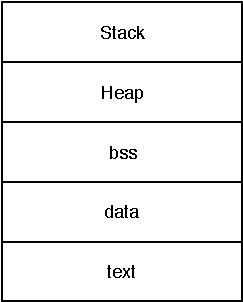
\includegraphics[]{assets/memory.pdf}
    \caption{\label{fig:kernel-types}memory organization}
\end{figure}

\subsection{Static memory management}
%stack
By the time a program begins to execute, there must be some specific blocks of memory reserved for its use.
This includes, for instance, the memory containing the program's own code.
Morever, every static variable must have a specific memory reserved.

The static memory allocation is predetermined by the compiler
    and will always be reserved for the program in the same manner at the beginning of every run.

This part of the memory operates as a \textit{stack} or last-in first-out (LIFO) queue.
The area of memory available for the use of the program will shrink and grow following the execution of the program,
which makes it very fast and efficient with no fragmentation.
%explain fragmentation?

\subsection{Dynamic memory management}
%heap
Sometimes, fixed memory size can be a problem.
Static memory does not allow allocation of memory beyond what is declared initially.
The \textit{heap} serves this purpose.
It is a large pool of memory which must be explicitly managed by the programmer.
It has no guarantee of efficient use of space, memory may become fragmented over time as blocks of memory are reallocated.

It may be tedious for the inexperienced programmer to manage the heap
    but it allows a more flexible and shareable pool of memory for an efficient programming.
To allocate memory on the heap, one must use \textit{malloc()} or \textit{calloc()} from the C code library stdlib.h (when available).
There are multiple algorithms to allocate memory when calling these functions.
The most common ones are presented below\cite{mem-mgmt-algo}.

% conventional algorithms
\subsubsection{Sequential fit algorithm}
For this memory management algorithm, a single linkedvlist contains the unallocated blocks of memory.
When needed, they are allocated using different policies:
\begin{itemize}
    \item First fit: returns the first block large enough from the list.
    \item Next fit: similar to first fit but starts where the pointer was left off at the previous iteration.
    \item Best fit: research through the whole list and returns the smallest block large enough to meet the request.
    \item Worst fit: returns the largest block from the list.
\end{itemize}

\subsubsection{Buddy allocator algorithm}
This algorithm makes use of an array of linked lists.
Each list from the array owns blocks of a distinct size.
When requested, the buddy allocator algorithm finds the smallest but large enough block to meet the requirement from the array.
It then picks one of the block from this position in the array.

If the list is empty at the position where the best fitting block is located, it goes to the next position in the array
and splits a block from this list to fill the empty position.
The opposite can also be applied: two smaller blocks can be merged to obtain a bigger one.

\subsubsection{Indexed fit algorithm}
This algorithm makes use of an indexed data structure to implement the desired fit.
Some common data structures used for this algorithm are trees or hash tables.

\subsubsection{Bitmapped fit algorithm}
A bitmap representing the usage of the heap is created.
Each bit of the map corresponds to a part of the heap.
If a part is used, the bitmap is set to 1.
If not, it is set to 0.
Allocation is done by searching the bitmap for clear bits.

% unconventional algorithms?

%\subsection{Virtual Memory}